\chapter{Getting started}
\thispagestyle{fancy}
\label{ch:getting-started}



\hrule
\begin{itemize}
\footnotesize
\item[]{Aims:}
\begin{itemize}
\item{to understand differences between commonly used local search methods;}
\item{to be aware of the assumptions in the linear approximation of parameter uncertainty:}
\item{to experience the limitations of local search methods for complex response surfaces;}
\item{to be aware of the existence of multiple minima in complex response surfaces;}
\item{to acknowledge the added value of global search methods;}
\item{to understand the need for efficient search methodologies.}
\end{itemize}
\end{itemize}
\hrule
\vspace{1em}

\section{Slug injection: manual calibration}

A classic method in hydrology for determining the transmissivity and storage coefficient of an aquifer is called the slug test. A known volume of water $Q$~[\textsf{m$^3$}] (the slug) is injected into a well, and the resulting effect on the head $h$~[\textsf{m}] (i.e.~water table elevation) at an observation well a distance $d$~[\textsf{m}] away from the injection is monitored at times $t$~[\textsf{hr}]. The measured head typically increases rapidly and then decreases more slowly. We wish to determine the storage coefficient $S$~[\textsf{m$^3\cdot{}$m$^{-3}$}] (a measure of the ability of the aquifer to store water) and the transmissivity $T$~[\textsf{m$^2\cdot{}$hr$^{-1}$}] (a measure of the ability of the aquifer to conduct water). The mathematical model for the slug test is:
\begin{equation}
\label{eq:slug-inj}
h=\frac{Q}{4\cdot{}\pi\cdot{}T\cdot{}t}e^{-d^2\cdot{}S/(4\cdot{}T\cdot{}t)}
\end{equation}



\smallq{Use the MATLAB editor to open `mancal\_sluginj.m' from `./exercises/manual-calibration-slug-injection/'. Run the script by pressing F5. A Graphical User Interface will appear. Use this interface to calibrate parameters $S$ and $T$ of Equation~\ref{eq:slug-inj}. Assume $Q$~=~50~[\textsf{m$^3$}] and $d$~=~60~[\textsf{m}].}

\smallq{How do $S$ and $T$ affect the simulated pressure head?}

Since this is a 2-parameter problem, we can easily visualize the objective function. Run `respsurf.m'. The objective function is the sum of squared residuals.

\smallq{Were you able to identify the ``optimal'' model parameters using manual calibration?}

\smallq{Looking at the response surface (Figure~\ref{fig:respsurf-sluginj}), do you think that the optimal model parameters are correlated?}
\begin{figure}[htbp]
  \centering
    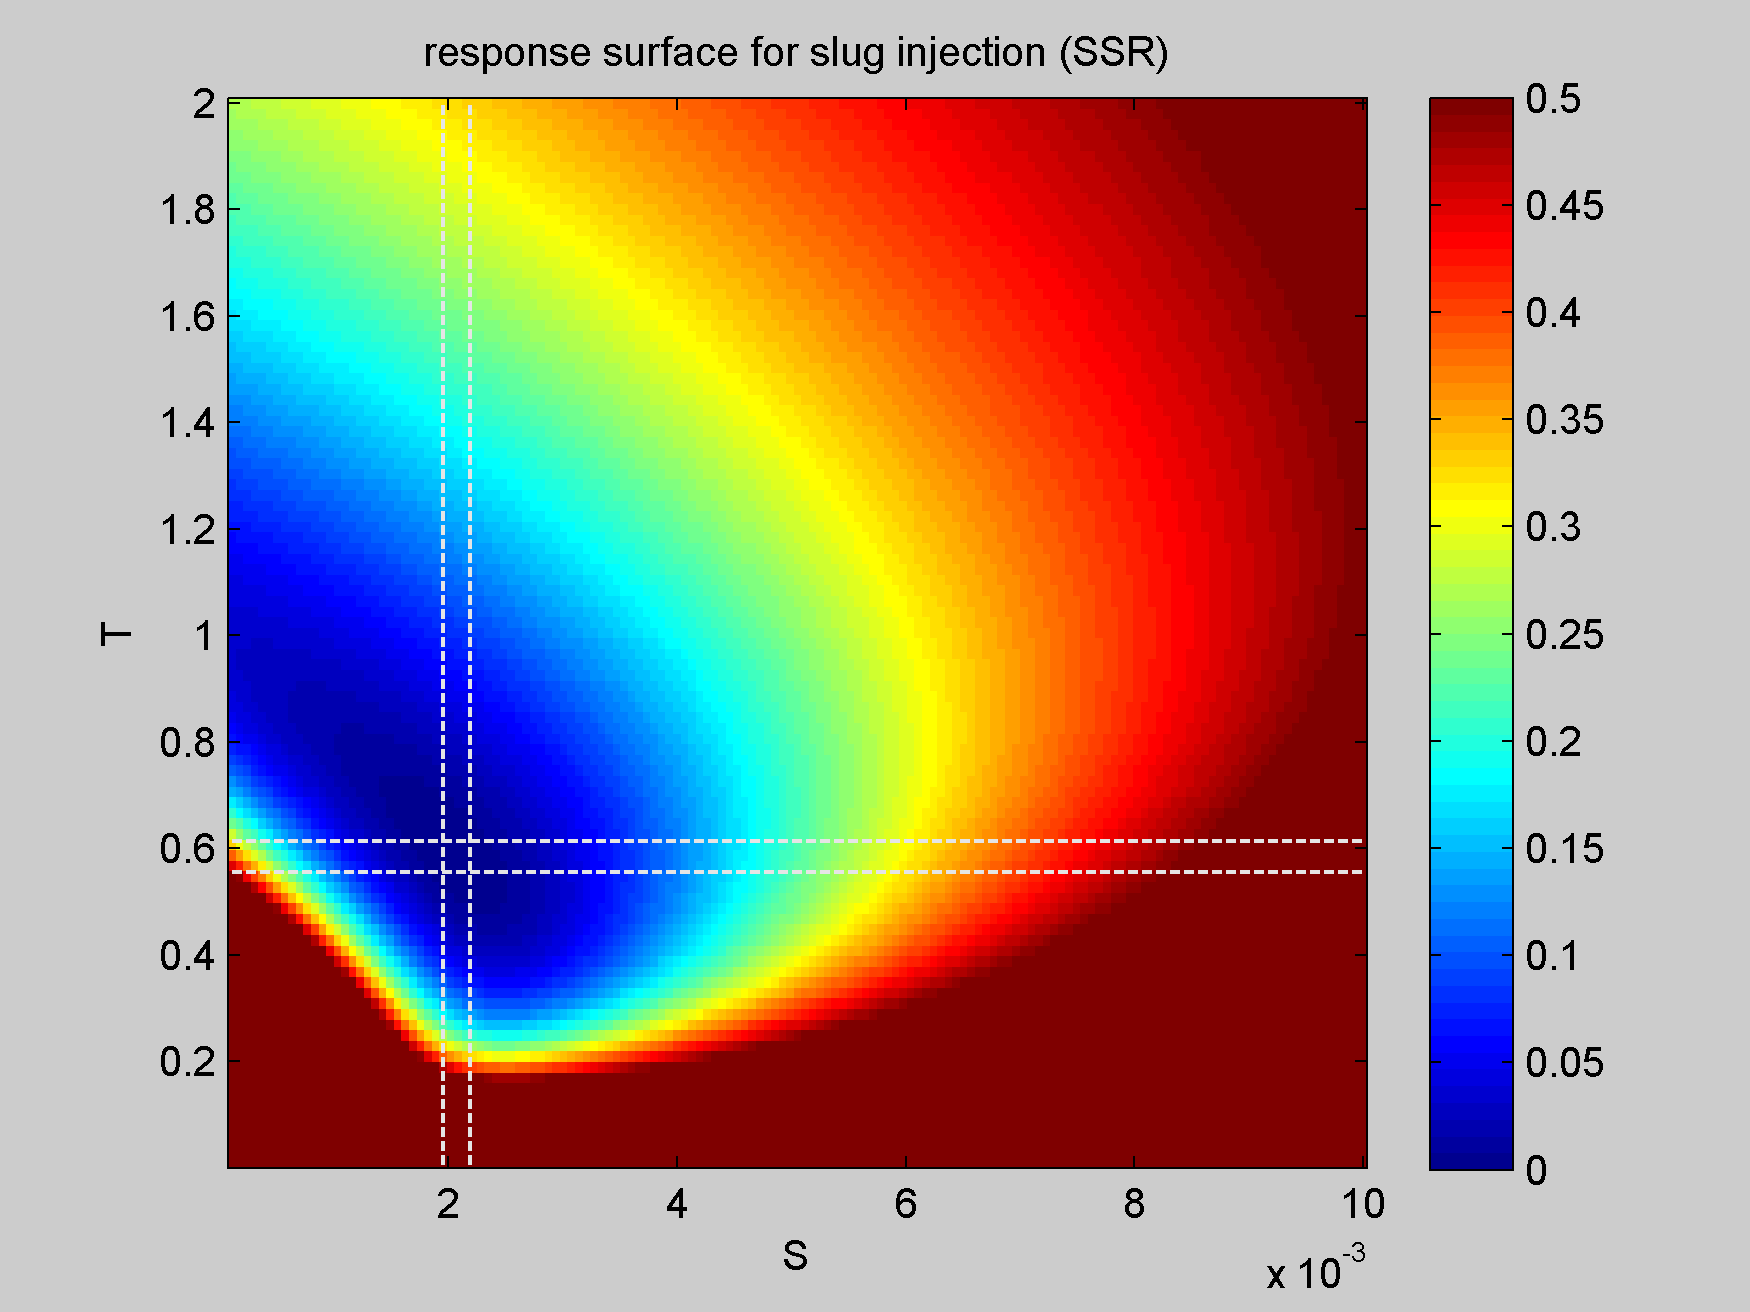
\includegraphics[width=1.0\textwidth]{./eps/converted/respsurf-sluginj}
  \caption{Response surface for the slug injection test. Dotted lines represent the 95\% confidence interval of the model parameters when the standard deviation of the head measurement is 0.01~[\textsf{m}].}
  \label{fig:respsurf-sluginj}
\end{figure}


\smallq{The dotted lines in Figure~\ref{fig:respsurf-sluginj} indicate the 95\% confidence intervals of the model parameters when the standard deviation of the head measurement is 0.01~[\textsf{m}]. Do you think this is a reasonable approximation for this nonlinear problem?}


\section{Optimization using local methods}

\subsection{Gauss-Newton and Levenberg-Marquardt}

\smallq{Two algorithms---Gauss-Newton (GN) and Levenberg-Marquardt (LM)--have been implemented to automatically find the optimal parameters for the slug test. To run these algorithms for the slug test problem, set your work directory to `./exercises/local-methods-sluginj'. This directory contains a function that performs a Gauss-Newton as well as a Levenberg-Marquardt optimization. This function requires an input argument containing a starting point (e.g.~\mcode{[0.15,0.4]}). For each method, the function returns an array with a record of parameter sets and their objective score. You can call the function from the command line using:

\mcode{[P_GN,P_LM]=Run_Optimization([0.15,0.4]);}
}



\smallq{Have a look at the code and interpret the output.}

\smallq{How quickly does the GN method converge?}

\smallq{How does this compare to the LM method?}

\smallq{Play around with different starting points for the two algorithms. Does the GN method always converge to the optimum? What about the convergence of the LM method?}

\smallq{Find a starting point where the GN and LM methods differ and study the iterations in detail (\mcode{P_GN} and \mcode{P_LM}).}

\smallq{What is the key difference between the iterations of the GN and LM method?}


\subsection{Multi-start simplex}

HYMOD \citep{boyl-gupt-soro2000} is a simple rainfall-runoff model with 5 model parameters (see Figure~\ref{fig:hymod}).

\begin{figure}[htbp]
  \centering
    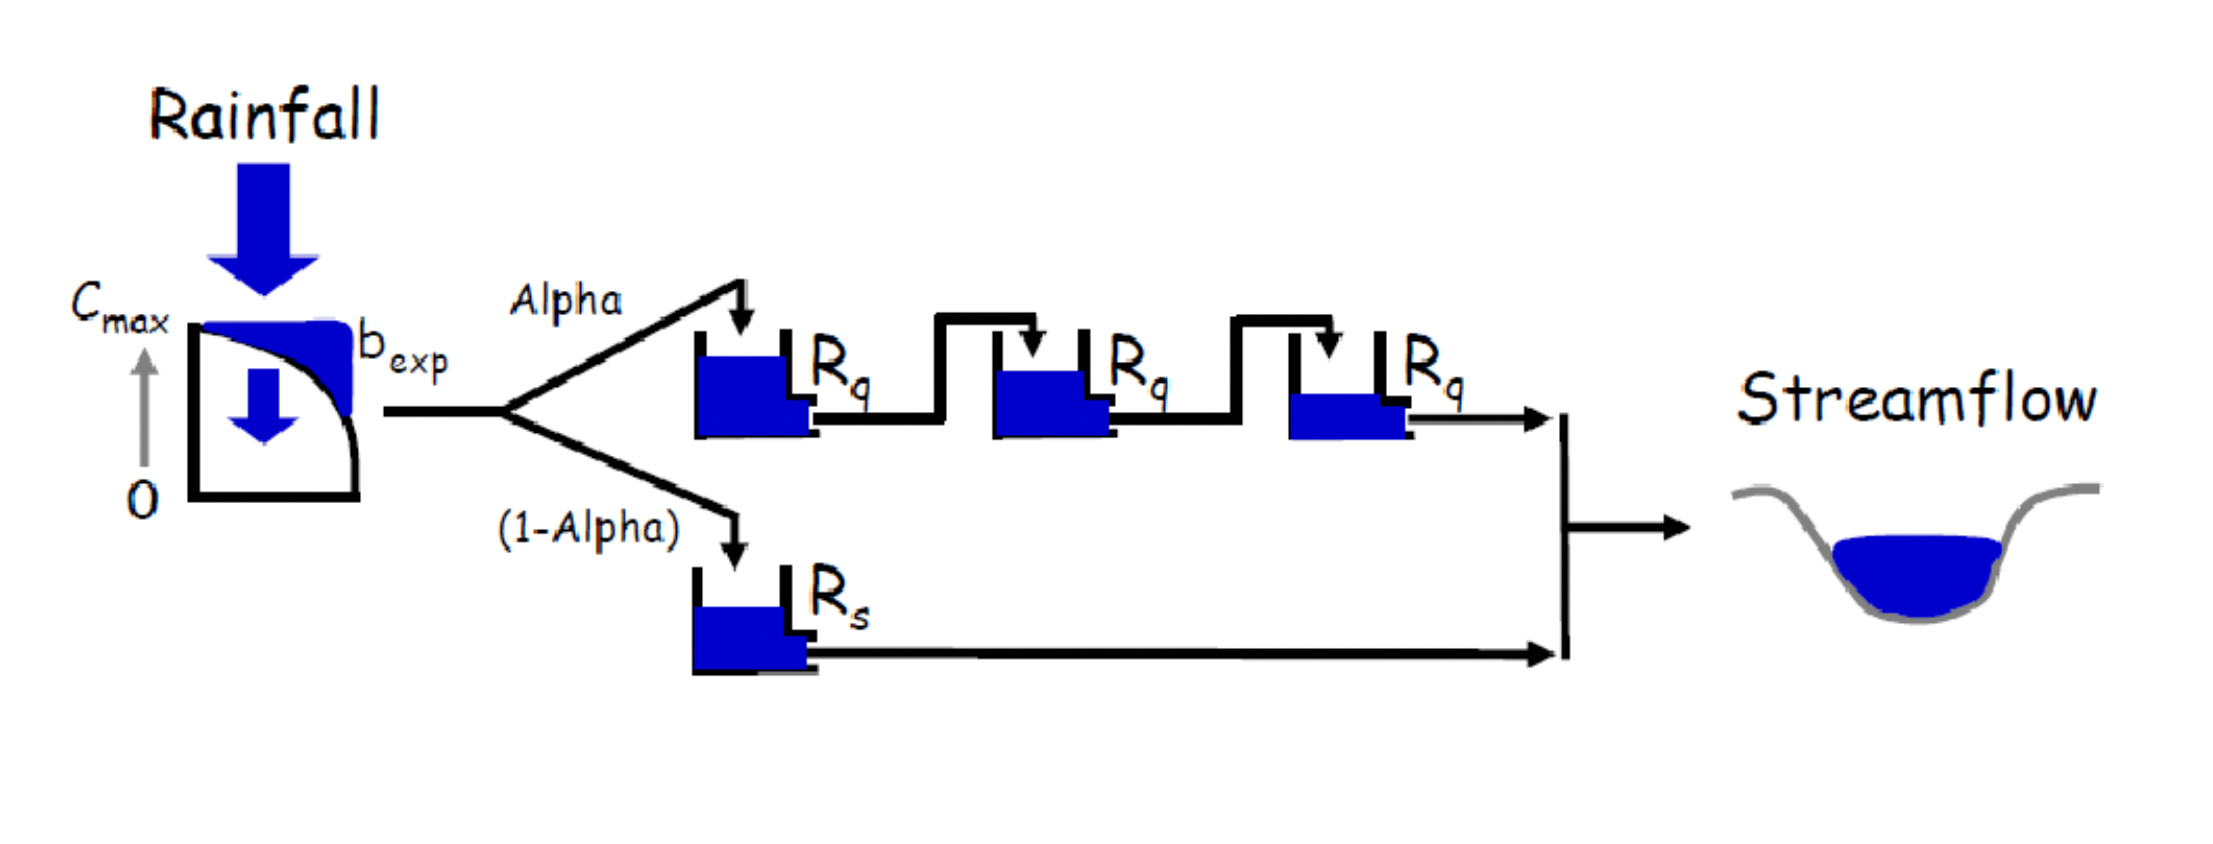
\includegraphics[width=1.0\textwidth]{./../eps/converted/hymod}
  \caption{Structure of the HYMOD rainfall-runoff model.}
  \label{fig:hymod}
\end{figure}
\begin{tabular}{ll}
with:&&\\
$C_{max}$&Maximum storage of the watershed\\
$b_{exp}$&Spatial variability of soil moisture capacity\\
$Alpha$&Partitioning factor of excess rainfall into slow and quick flow\\
$R_{s}$&Residence time of the slow tank\\
$R_{q}$&Residence time of the quick tanks\\
\end{tabular}

In this section, we will use a multi-start simplex \citep{neld-mead1965} to optimize the parameters of the HYMOD model. Specifically, we investigate whether the objective function (SSR) of this model has local minima that may complicate the use of local optimization methods such as Gauss-Newton, or Levenberg-Marquardt. To do this, 20 simplex runs are started from randomly determined starting points, which are iterated until convergence is achieved.

\smallq{First, have a look at the code of `Multistart\_Simplex.m' in `./exercises/local-methods-hymod/'. As you can see, the code uses the built-in MATLAB function \mcode{fminsearch}, which is an implementation of the simplex search algorithm. Run \mcode{Multistart\_Simplex} (it'll run for a few minutes). Store the output by copying and pasting into a PowerPoint presentation.}

\smallq{Do all the Simplex runs converge to the same point in the parameter space?}

\smallq{What does this tell you about the presence of local minima?}

\smallq{For the slug injection test, we visualized the response surface. Can we make a similar figure here?}

\smallq{When you look at the results of the simulations with optimized parameters, why do you see just 3 or 4 time series and not 20?}

\smallq{How do you value the results of the various models?}


\smallqo{In the previous exercise, a relatively short data set (3 months) was used to calibrate HYMOD. Extend the calibration period to 12 months by changing the values of \mcode{Extra.calPeriod} in  \mbox{`Multistart\_Simplex.m'} and run the optimization again.}

\smallqo{For this new subset of data, why did the number of local minima increase or decrease?}

\smallqo{What is the quality of the model runs corresponding to the local minima?}

\smallqo{If we discard the poor models, can you give an interpretation why these local minima occurred?}





\section{Global methods: Differential Evolution}


Differential Evolution~\citep{stor-pric1997} is a basic global optimization algorithm that uses a population of points in the parameter space to find the global maximum (minimum, if appropriate) of an objective function. Generally speaking, the population's properties are used to generate more points in those parts of the parameter space which are most promising with regard to yielding the global optimum.

\smallq{Use the MATLAB editor to open `./exercises/differential-evolution/respsurf.m'. This script contains a few lines of code to help you get started on your algorithm. Run the script to visualize the response surface for the benchmark function `6' (Shifted Rosenbrock's  Function) for \mcode{x = [65:0.1:80]} and \mcode{y = [35:0.1:45]} (Figure~\ref{fig:respsurf-rosenbrock}).}
\begin{figure}[htbp]
  \centering
    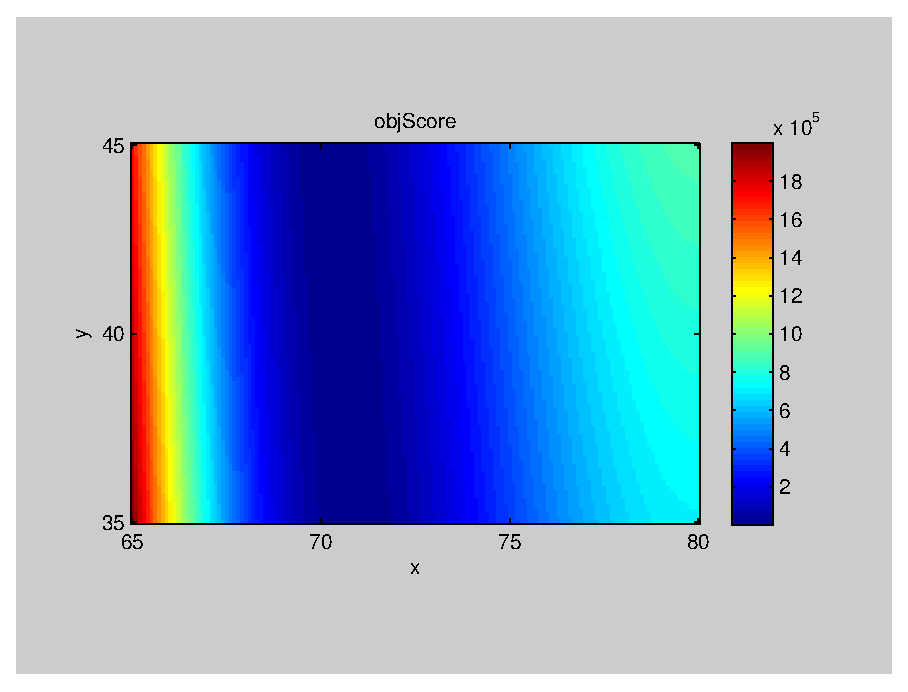
\includegraphics[width=1.0\textwidth]{./../eps/respsurf-rosenbrock.eps}
  \caption{Response surface for the shifted Rosenbrock function.}
  \label{fig:respsurf-rosenbrock}
\end{figure}

The \mcode{benchmark_func} function offers not just 1, but 25 functions that can be visualized in the same way as you already did for the Rosenbrock function. You can choose different functions by changing the \mcode{funcFlag}. Each function has its own limits on the parameter space (see Table~\ref{tab:benchmark-func-data}).

\begin{table}[t]
\centering
\scriptsize
\begin{tabular}{lp{9cm}l}
\mcode{funcFlag}&\textbf{description}&\textbf{limits}\\
\multicolumn{3}{l}{Unimodal Functions (5):}\\
1  &Shifted Sphere Function                                                              & [-100,100]\\
2  &Shifted Schwefel's Problem 1.2                                                       & [-100,100]\\
3  &Shifted Rotated High Conditioned Elliptic Function                                   & [-100,100]\\
4  &Shifted Schwefel's Problem 1.2 with Noise in Fitness                                 & [-100,100]\\
5  &Schwefel's  Problem 2.6 with Global Optimum on Bounds                                & [-100,100]\\
\multicolumn{3}{l}{Multimodal Functions (20):}\\
\multicolumn{3}{l}{Basic Functions (7):}\\
6  &Shifted Rosenbrock's Function                                                        & [-100,100]\\
7  &Shifted Rotated Griewank's Function without Bounds                                   & [0,600]\\
8  &Shifted Rotated Ackley's Function with Global Optimum on Bounds                      & [-32,32]\\
9  &Shifted Rastrigin's Function                                                         & [-5,5]\\
10  &Shifted Rotated Rastrigin's  Function                               & [-5,5]\\
11  &Shifted Rotated Weierstrass Function                                & [-0.5,0.5]\\
12  &Schwefel's  Problem 2.13                                            & [-100,100]\\
\multicolumn{3}{l}{Expanded Functions (2):}\\
13  &Expanded Extended Griewank's  plus Rosenbrock's  Function (F8F2)                    & [-3,1]\\
14  &Expanded Rotated Extended Scaffe's  (F6)                                & [-100,100]\\
\multicolumn{3}{l}{Hybrid Composition Functions (11):}\\
15  &Hybrid Composition Function 1                                       & [-5,5]\\
16  &Rotated Hybrid Composition Function 1                               & [-5,5]\\
17  &Rotated Hybrid Composition Function 1 with Noise in Fitness                     & [-5,5]\\
18  &Rotated Hybrid Composition Function 2                               & [-5,5]\\
19  &Rotated Hybrid Composition Function 2 with a Narrow Basin for the Global Optimum    & [-5,5]\\
20  &Rotated Hybrid Composition Function 2 with the Global Optimum on the Bounds         & [-5,5]\\
21  &Rotated Hybrid Composition Function 3                           & [-5,5]\\
22  &Rotated Hybrid Composition Function 3 with High Condition Number Matrix         & [-5,5]\\
23  &Non-Continuous Rotated Hybrid Composition Function 3                        & [-5,5]\\
24  &Rotated Hybrid Composition Function 4                               & [-5,5]\\
25  &Rotated Hybrid Composition Function 4 without Bounds                            & [-2,5]\\
\end{tabular}
\caption{}
\label{tab:benchmark-func-data}
\end{table}

\smallq{Experiment with different functions to get some idea of what their response surfaces look like.}

%\hspace*{0.01mm}
%\vfill
%\hspace*{0.01mm}


\needspace{8\baselineskip}
In the next few exercises, you will write your differential evolution algorithm. We will take you through these basic steps:
\begin{enumerate}
\item{generate the initial sample;}
\item{assign the initial sample to a new array \mcode{parents};}
\item{for each sample in \mcode{parents}, calculate the corresponding objective score;}
\item{use \mcode{parents} to calculate new \mcode{proposals};}
\item{for each sample in \mcode{proposals}, calculate the corresponding objective score;}
\item{accept either a sample from \mcode{proposals} or the corresponding sample from \mcode{parents} as the child, thus making an array \mcode{children} of the same size as \mcode{parents};}
\item{assign \mcode{children} to \mcode{parents} for the next generation, and go back to step 4.}
\end{enumerate}

\smallq{Save your \mcode{respsurf} script under a new name `runDiffEvo.m'.}

\smallq{Extend `runDiffEvo.m' by creating an array \mcode{parents}, which has \mcode{nPop=50} rows, each of which represents a uniform random sample from the parameter space. \mcode{parents} has \mcode{nDims+1} columns, i.e. the number of dimensions for which you want to solve \mcode{benchmark_func} plus one column to store the objective score. Refer to Table~\ref{tab:benchmark-func-data} for the parameter space limits. For now, stick with \mcode{nDims=2} and \mcode{funcFlag=6}, but you can change that later.}

\smallq{Calculate the last column of \mcode{parents} by running the objective function for each row.}

\smallq{Generate the \mcode{proposals} array (same size as \mcode{parents}). To do this, select the first sample from \mcode{parents}, as well as three other samples (\mcode{r1}, \mcode{r2}, \mcode{r3}), chosen at random from \mcode{parents} (MATLAB's built-in function \mcode{randperm} can be useful for this). The proposal is calculated as the position of the parent + F*\mcode{dist1} + K*\mcode{dist2}, in which  \mcode{dist1} is the distance between the parent and \mcode{r1}, \mcode{dist2} is the distance between \mcode{r2} and \mcode{r3}, and F and K are settings that are part of the Differential Evolution algorithm. In the literature, F=0.6 and K=0.4 are common. Repeat for all samples in parents.}

\smallq{For each member in \mcode{proposals}, calculate the objective score.}

\smallq{Determine whether to choose the $i^{th}$ sample of \mcode{parents} or the $i^{th}$ sample of \mcode{proposals}, depending on which one has a better objective score. Assign to the $i^{th}$ row in a new array \mcode{children}.}

\smallq{Assign \mcode{children} to \mcode{parents} for the next generation.}

\smallq{Wrap most of the above steps in a \mcode{for} loop, such that your script will repeatedly generate new (and hopefully better) children for 250 generations.}

\smallq{It's a little bit difficult to see if your script is doing what it is supposed to be doing, so you need to do some visualization. Copy and paste from `vis-helper.txt' to create a figure similar to Figure~\ref{fig:diffevo-result}.}

\begin{figure}[htbp]
  \centering
    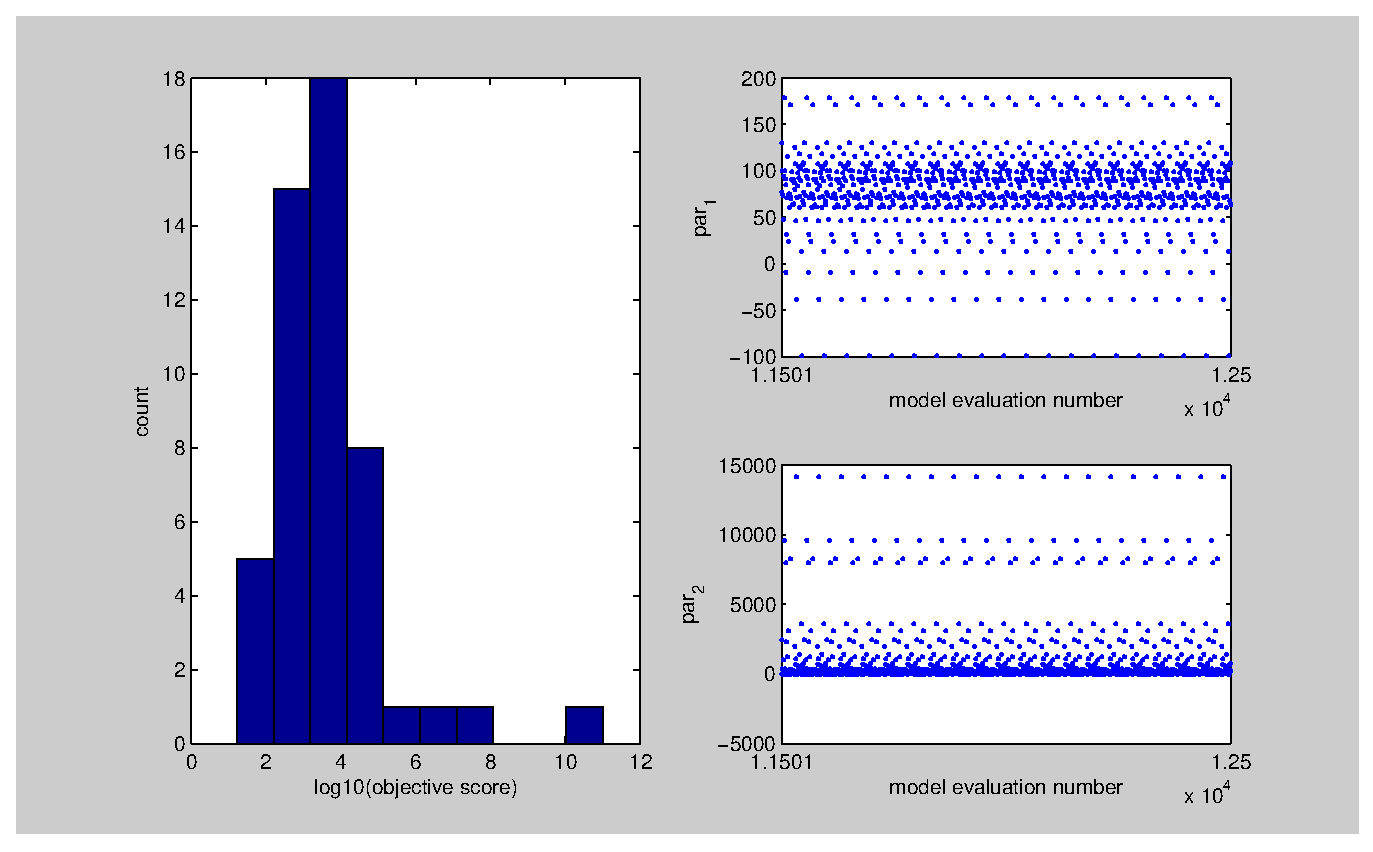
\includegraphics[width=1.0\textwidth]{./../eps/diffevo-result.eps}
  \caption{Visualization results for the Shifted Rosenbrock function after 250 generations of 50 samples each, optimized using the Differential Evolution algorithm.}
  \label{fig:diffevo-result}
\end{figure}



\smallq{During the optimization, you may notice that there are some points that are really persistent, even though they are well away from the global optimum. Explain why these points are so persistent.}

\smallq{The histogram in Figure~\ref{fig:diffevo-result} is bimodal. How does that relate to the answer to the previous question?}




